\documentclass[11pt,letterpaper]{article}
\usepackage[T1]{fontenc}
\usepackage{lmodern}
\usepackage[margin=1in,headheight=15pt]{geometry}
\usepackage{amsmath,amssymb,amsthm,mathtools}
\usepackage{microtype,booktabs,longtable,array,enumitem}
\usepackage{needspace}
\usepackage{xcolor,graphicx,fancyhdr}
\usepackage[hyphens]{url}
\definecolor{ink}{HTML}{18384E}
\definecolor{accent}{HTML}{006B72}
\usepackage[colorlinks=true,linkcolor=ink,citecolor=accent,urlcolor=accent]{hyperref}
\usepackage{bookmark}
\hypersetup{pdftitle={Stopping Sets, Saturated Bundles, and Exact Raw Cancellation},
  pdfauthor={Research continuation for Vladimir Reshetnikov; development with ChatGPT},
  pdfsubject={Certified local improvements for the ProveIt unknot-recognition program}}
\usepackage{listings}
\lstset{basicstyle=\small\ttfamily,breaklines=true,columns=fullflexible,
  keepspaces=true,frame=single,rulecolor=\color{black!15},xleftmargin=.5em,
  xrightmargin=.5em,showstringspaces=false}
\setlist{topsep=5pt,itemsep=3pt,parsep=0pt}
\setlength{\emergencystretch}{3em}
\newtheorem{theorem}{Theorem}[section]
\newtheorem{lemma}[theorem]{Lemma}
\newtheorem{proposition}[theorem]{Proposition}
\newtheorem{corollary}[theorem]{Corollary}
\theoremstyle{definition}
\newtheorem{definition}[theorem]{Definition}
\newtheorem{example}[theorem]{Example}
\theoremstyle{remark}
\newtheorem{remark}[theorem]{Remark}
\newcommand{\NN}{\mathbb N}
\newcommand{\supp}{\operatorname{supp}}
\newcommand{\Stop}{\operatorname{Stop}}
\newcommand{\capTwo}{\operatorname{cap}_2}
\newcommand{\poly}{\operatorname{poly}}
\newcommand{\rk}{\operatorname{rank}}
\newcommand{\per}{\operatorname{per}}
\newcommand{\raw}{\mathsf{raw}}
\newcommand{\code}[1]{\texttt{\detokenize{#1}}}
\pagestyle{fancy}
\fancyhf{}
\fancyhead[L]{\small\textcolor{ink}{ProveIt: unknot recognition}}
\fancyhead[R]{\small Stopping cores and saturated bundles}
\fancyfoot[C]{\thepage}
\renewcommand{\headrulewidth}{.3pt}
\title{\textcolor{ink}{Stopping Sets, Saturated Bundles,\\and Exact Raw Cancellation}\\[.5em]
\large A certified performance improvement for the ProveIt unknot-recognition program}
\author{Research continuation prepared for Vladimir Reshetnikov\\
\small Mathematical development and implementation with ChatGPT}
\date{12 October 2026\\\small Source revision \texttt{704600626606a9097cfd89d4e3d2bbc63c8dd1cb}}
\begin{document}
\maketitle
\begin{abstract}
We study two specific bottlenecks in the source-certified normal-cut pipeline.
First, we prove that complete positive raw cancellation of an arbitrary
rectangular nonnegative incidence matrix is equivalent to deletion of unit
column leaves. A nonempty stopping set survives every positive Schur update,
which proves completeness of a sparse source algorithm and provides a short
obstruction certificate. The canonical peeling construction is classical in
coding theory; the persistence argument and its use in geometric cancellation
are the contributions developed here. This strengthens the repository's
square-only completeness statement, removes repeated matrix scans, and shows
that survivor-set enumeration is unnecessary for this decision problem.

Second, we continue the incoming one-two-handle theorem for saturated interval
bundles. Their residual attaching curves have a source-computable unsigned
incidence on old core cocores, while every added band column is even and can
never supply a raw singleton pivot. Thus arbitrarily large numerical base
genus can be excluded from cancellation search. We implement a whole-cut
certificate that combines the old core rows with one aggregate row per
saturated base and independently verifies the resulting handlebody census.
All geometric conclusions are tied to authenticated embedded source charts.

The package includes proofs, a repository integration patch with updated files,
independent checkers, exhaustive algebraic tests, source-cut comparisons,
paired measurements, and a focused research agenda. The improvement concerns
supplied-cut certification. It neither implements nor proves a general
quasi-polynomial unknot recognizer; surface production, transported boundary
patterns, and total hierarchy work remain separate obligations.
\end{abstract}
\clearpage
\tableofcontents
\clearpage
\section{Scope, source audit, and the research question}
\label{sec:position}

\subsection{What this continuation changes}

The immediate mathematical question is precise. After choosing a spanning
forest in an authenticated geometric handle core, let $n_{ih}$ count the
actual intersections of the $i$th two-handle attaching curve with the
cocore of the $h$th surviving one-handle. The existing implementation accepts
a positive singleton pivot $n_{rg}=1$ and updates
\begin{equation}\label{eq:positive-pivot}
 n'_{ih}=n_{ih}+n_{ig}n_{rh}\qquad(i\ne r,\ h\ne g).
\end{equation}
It seeks to remove every two-handle. We ask whether finding a successful
order, including its surviving one-handles, actually requires branching.

The answer is no. A unit column leaf is a column whose total incidence on
the live rows is exactly one. Its pivot has no fill in the remaining rows.
Repeatedly deleting such leaves is complete for the entire positive raw
model, even on rectangular matrices. A stopped nonempty row set is a
certificate that \emph{no} positive pivot order can finish. This is a stronger
statement than a failure of a chosen order.

The second question concerns an interval-bundle component whose entire base
boundary is attached to the core. Previous work localizes its obstruction
to a single residual two-handle, but the number of added one-handles can
be very large. We show that these added columns need never be generated
for raw cancellation: they are even. The only relevant row is the aggregate
of the source boundary-circle incidences on old core cocores. This connects
the exact matrix theorem to a new source-bound geometric operator.

\subsection{The pinned repository and incoming reports}

The inspected source is the public
\href{https://github.com/VladimirReshetnikov/ProveIt}{ProveIt repository},
at commit
\begin{center}\texttt{704600626606a9097cfd89d4e3d2bbc63c8dd1cb}.\end{center}
The target subtree is \path{Topology/UnknotRecognition}; the supplied
incoming directory contains four research archives\cite{repo,incoming}.
All source paths and hashes used for integration are retained in the package.

The maintained pipeline already includes compressed normal-cut cells,
parallelity bases and their ordered interfaces, source handle charts,
raw geometric cancellation, disk-base absorption, and a simultaneous
primitive-annulus rule. The latter uses a spare unattached base boundary
to supply dual disks. The incoming hierarchy report proves a more general
relative-band theorem for nonsaturated attachments and a one-two-handle
localization for each saturated base. We use these results as starting
points, give the needed geometry explicitly, and identify our additions.

\begin{longtable}{@{}>{\raggedright\arraybackslash}p{.28\textwidth}
>{\raggedright\arraybackslash}p{.36\textwidth}
>{\raggedright\arraybackslash}p{.29\textwidth}@{}}
\toprule
Source checkpoint & Existing result & Role in this report\\
\midrule\endhead
Maintained core cancellation & Saturated positive pivots; complete square
row-leaf test; rectangular capped planner & Replace repeated rectangular
scans and strengthen the completeness analysis\\
Maintained primitive annuli & A spare base boundary gives a simultaneous
geometric primitive family & Preserve this case and admit certain fully
attached bases\\
Incoming hierarchy kernels & Relative one-handles for nonsaturated bases;
one residual two-handle for each saturated base & Compute the residual old
incidences and eliminate all added even columns from search\\
Incoming disconnected tile kernels & Exact finite kernels for repeated
disconnected cubic tiles & Complementary terminal-pattern work; not rederived\\
Incoming moment-coded returns & Two-moment recovery of ordered boundary
first returns & Complementary interface optimization; not integrated here\\
Incoming sparse cut grammars & Composition of bounded-cut graph responses
through connected grammars & Complementary hierarchy-state work; not rederived\\
\bottomrule
\end{longtable}

The current min-fill rectangular planner deserves a correction, rather
than a false coverage claim. Its documentation calls it incomplete.
Our theorem shows that its particular zero-fill priority is already complete
for full raw row cancellation. The new algorithm therefore gives a simpler
proof, smaller search work and faster replay; it does not create previously
missing successes in that old raw model. New geometric coverage comes from
the saturated-bundle extension.

\subsection{The quasi-polynomial target and current primary sources}

The 109-page 2021 talk linked by the repository states a running time
$n^{O(\log n)}$\cite{lackenby-talk}. The shorter Oxford handout displays
$2^{O((\log n)^3)}$\cite{lackenby-oxford}. Both are quasi-polynomial, but they
are distinct bounds. We retain the stronger $n^{O(\log n)}$ expression as
the user's target and do not equate it with the handout's exponent.

Lackenby's July 2026 preprint\cite{lackenby-2026} presents a complete
hierarchy algorithm and efficient certificates, while reserving speed-up
for later work. Its Section 9 explicitly does not provide the precision
needed for a running-time estimate. Proposition 9.1 bounds iterations in
terms of hierarchy length $L$ and pattern-complexity bound $g$ by
$L(g+1)^L$. Theorems 14.1 and 14.4 concern efficient certification and
compressed cut structure. These results give important mathematical
infrastructure, but they do not turn an arbitrary local optimization into
the announced global time bound. Section~\ref{sec:hierarchy} records the
remaining obligations and the exact place of our operator.

\subsection{Prior art and the intended novelty claim}

Unit-column peeling and stopping sets have substantial prior art.
Richardson--Urbanke\cite[Appendix C]{richardson-urbanke} define stopping
sets on constraint rows, prove union closure, and identify the unique
maximal stopping set as the residual of degree-one-column elimination.
Di et al.\cite[Definition 1.1 and Lemma 1.1]{di-et-al} use the corresponding
criterion for erasure decoding, including a multigraph formulation.
Uniquely restricted matchings provide a related matrix language\cite{urm}.
We do not claim to invent these constructions.

The mathematical additions developed here are the explicit persistence
identity under \eqref{eq:positive-pivot}, its complete geometric raw-cancellation
consequence, the source-incidence formula for saturated residual curves,
and the resulting parity exclusion of unexpanded band handles. The code
contribution is a native producer and separate replay path for these
results. The asserted novelty is relative to the inspected project and
the primary sources just identified. No claim of exhaustive bibliographic
priority is needed for the proofs or implementation.

\subsection{Notation and conventions}

All matrices have entries in $\NN=\{0,1,2,\ldots\}$. Counts are unsigned
geometric counts, not exponent sums. A row denotes an attaching curve
or a residual saturated-bundle relation, and a column denotes a one-handle
cocore. We allow zero rows, empty matrices and unused columns. A full
cancellation removes all rows; it need not remove all columns.

For a source triangulation, $T$ denotes its tetrahedron count, $P$ its
number of active interface ports, and $B$ the aggregate bit-length parameter
of its binary coordinates and topology counters. For a finite sparse
matrix, $m,n,I$ denote its row count, column count and number of nonzero
entries. Distinguishing $I$ from the sum of numerical entries is essential:
neither large multiplicities nor large base genus are expanded.

\section{Stopping sets survive positive raw cancellation}
\label{sec:stopping}

\begin{definition}[Positive raw pivot]
Let $N=(n_{ih})$ be a nonnegative integral matrix. A positive raw pivot at
$(r,g)$ is allowed when $n_{rg}=1$. It deletes row $r$ and column $g$ and
replaces the other entries by \eqref{eq:positive-pivot}. A full raw
cancellation is a finite sequence of such pivots that removes every row.
\end{definition}

The adjective positive refers to the plus sign in the update. In particular,
this operation is not Gaussian elimination over a field. It records a
geometric disk-slide model before any subsequent reduction of intersections.

\begin{definition}[Stopping set]
A nonempty set $R$ of rows of $N$ is a stopping set if, for each column $h$,
\begin{equation}\label{eq:stopping}
 S_h(R):=\sum_{i\in R}n_{ih}\in\{0,2,3,\ldots\}.
\end{equation}
Thus no column has exactly one crossing into $R$. The empty set is admitted
when discussing unions, but it is never an obstruction certificate.
\end{definition}

A coefficient two in a single row counts as two crossings. Replacing the
matrix by its Boolean support would lose precisely this distinction.

\begin{theorem}[Persistence under every positive pivot]
\label{thm:persistence}
Suppose $R$ is a stopping set of $N$ and a positive raw pivot is performed
at $(r,g)$. If $r\notin R$, then $R$ is a stopping set of the new matrix.
If $r\in R$, then $R\setminus\{r\}$ is nonempty and is a stopping set of
the new matrix. Consequently a matrix with a nonempty stopping set admits
no full raw cancellation.
\end{theorem}

\begin{proof}
First let $r\notin R$. For every surviving column $h$,
\[
 S'_h(R)=S_h(R)+S_g(R)n_{rh}.
\]
Each summand is either zero or at least two, because $S_h(R)$ and $S_g(R)$
have that property. Their sum therefore cannot equal one.

Now let $r\in R$. Since $n_{rg}=1$, the stopping condition at $g$ forces
$S_g(R)\ge2$. Put
\[
 k=\sum_{i\in R\setminus\{r\}}n_{ig}=S_g(R)-1\ge1.
\]
In particular $R\setminus\{r\}$ is nonempty. For any surviving $h$,
\begin{align}
 S'_h(R\setminus\{r\})
 &=S_h(R)-n_{rh}+k n_{rh}\notag\\
 &=S_h(R)+(k-1)n_{rh}.\label{eq:stopping-persistence}
\end{align}
If $S_h(R)=0$, nonnegativity implies $n_{rh}=0$ and the expression is zero.
If $S_h(R)\ge2$, it remains at least two. This proves persistence in both
cases. Inductively, a nonempty stopping set survives every prefix of a
positive pivot sequence, so such a sequence cannot remove every row.
\end{proof}

The short identity \eqref{eq:stopping-persistence} is useful because it
rules out \emph{all} positive pivot orders directly. It does not presume
a matching, a chosen survivor set or a deterministic producer.

\begin{definition}[Column-leaf deletion]
A column $g$ is a unit leaf in the current matrix if
$\sum_i n_{ig}=1$. There is then a unique incident row $r$, its entry is
one, and its positive pivot has no fill: all surviving $n_{ig}$ vanish.
A column-leaf deletion removes this row and column.
\end{definition}

\begin{theorem}[Complete rectangular raw cancellation]
\label{thm:complete}
For every finite nonnegative integral matrix $N$, the following are equivalent:
\begin{enumerate}[label=(\roman*)]
\item $N$ admits a full positive raw cancellation;
\item $N$ has no nonempty stopping set;
\item every maximal sequence of unit column-leaf deletions removes all rows;
\item some sequence of unit column-leaf deletions removes all rows.
\end{enumerate}
In particular, deciding full raw cancellation requires no branching over
pivot orders or over the columns that will survive.
\end{theorem}

\begin{proof}
Theorem~\ref{thm:persistence} gives (i)$\Rightarrow$(ii).
Run any maximal column-leaf sequence. If rows remain, call their set $R$.
Every undeleted column has total zero or at least two on $R$, because the
sequence is maximal. Each deleted column had only its designated row live
when it was removed; hence its total on the final $R$ is zero. No fill has
ever occurred. Therefore $R$ is a stopping set of the original matrix.
This proves (ii)$\Rightarrow$(iii). Implication (iii)$\Rightarrow$(iv) is
immediate, and every leaf deletion is a valid raw pivot, giving
(iv)$\Rightarrow$(i).
\end{proof}

\begin{corollary}[A canonical obstruction]
\label{cor:canonical}
There is a unique largest stopping set, with the empty set allowed.
Every maximal column-leaf sequence leaves exactly this row set, denoted
$\Stop(N)$. Thus the residual row set is independent of tie choices,
although pivot columns and successful schedules need not be unique.
\end{corollary}

\begin{proof}
The union of stopping sets is a stopping set: if a column meets the union,
it meets one constituent set and already has total at least two there.
Because there are finitely many rows, their union gives the largest set.
No column leaf can delete a row in an extant stopping set, since that set
would have column sum one. Hence every original stopping set lies in the
final residual. The proof of Theorem~\ref{thm:complete} shows that the
residual is itself a stopping set. The two containments prove the claim.
\end{proof}

This canonical peeling statement is the classical stopping-set phenomenon
identified in the prior-art discussion. The additional persistence theorem
explains why the same obstruction remains valid when the allowed operations
are enlarged from leaf deletions to all positive raw pivots.

\subsection{Exact saturation and sparse representation}

\begin{lemma}[Saturation at two is exact for the model]
\label{lem:saturation}
The map $\capTwo(a)=\min(2,a)$ preserves addition and multiplication when
the target operations are capped at two. It preserves the singleton
predicate and the stopping-set predicate. It therefore preserves the
existence of a full positive raw cancellation.
\end{lemma}

\begin{proof}
For $a,b\in\NN$, both
$\min(2,a+b)=\min(2,\min(2,a)+\min(2,b))$ and
$\min(2,ab)=\min(2,\min(2,a)\min(2,b))$ follow by splitting into whether
the result is zero, one or at least two. The same identities commute
with \eqref{eq:positive-pivot}. A sum is one exactly when one summand is
one and all the others are zero, which is also unchanged by capping.
\end{proof}

Actual crossing multiplicities may consequently be arbitrarily large in
binary without changing the finite peeling state. Values zero, one and
at least two are all that the decision needs. This statement does not
authorize replacing a geometric count by a signed exponent sum.

\subsection{A matching interpretation, without a matching algorithm}

\begin{corollary}[Unit uniquely restricted row matching]
\label{cor:matching}
A full raw cancellation exists if and only if there is a set of $m$
columns whose $m\times m$ submatrix has permanent one. Equivalently,
the weighted bipartite incidence multigraph has a row-saturating matching
whose induced square subgraph has a unique perfect matching, all of whose
chosen edge multiplicities are one.
\end{corollary}

\begin{proof}
Suppose peeling removes all rows. Select the $m$ pivot columns and order
both rows and those columns by deletion time. A pivot column has its
diagonal entry one and no nonzero in any later row. Thus the selected
square matrix is triangular with unit diagonal. Its only nonzero
permanent term is the diagonal term.

Conversely, a nonnegative integral square matrix of permanent one has a
unique perfect matching with unit chosen entries. Orient an off-matching
incidence from its row's matched pair to the incident column's matched
pair. A directed cycle would give an alternating cycle and a second
perfect matching. The directed graph is therefore acyclic and has a
source. Its matched column has no incidence from other rows. Removing
that pair and repeating gives column-leaf deletion of the selected minor.
These are also column leaves in the full matrix, because the selected
minor includes every row. Other columns do not affect a leaf's column sum.
\end{proof}

There is no need to compute a permanent or to enumerate the selected
columns. The direct obstruction theorem supplies the complete algorithm.
The distinction between \emph{saturating all rows} and maximizing the
size of a partially constrained matching should be retained when comparing
this corollary with matching literature.

\subsection{Boundary cases and limits of the conclusion}

\begin{example}[A zero row]
A single all-zero row is a stopping set. A raw singleton cancellation
cannot remove its two-handle, even if that handle has some other geometric
disposal, such as a later two/three-handle cancellation. Three-handles are
outside the present model.
\end{example}

\begin{example}[Peeling is not maximum partial cancellation]
For
$N=\left(\begin{smallmatrix}1&1\\1&1\end{smallmatrix}\right)$, every
column has total two and no column leaf exists. A positive pivot can
nevertheless remove one row and leave the matrix $(2)$. Thus
$|\Stop(N)|$ is not the minimum number of rows attainable by an arbitrary
partial raw sequence. The theorem decides complete cancellation and gives
a canonical source obstruction; it does not optimize partial progress.
\end{example}

\begin{example}[A unimodular raw obstruction]\label{ex:unimodular}
The matrix
\[
 U=\begin{pmatrix}1&1\\1&2\end{pmatrix}
\]
has determinant one, but its entire row set is a stopping set. Every legal
first raw pivot leaves the single entry three. Signed linear algebra
therefore cannot replace the unsigned criterion. The group presentation
$\langle x,y\mid xy,xy^2\rangle$ is trivial, since the two equations give
$y=1$ and then $x=1$. Its raw occurrence matrix is $U$.

There is also a geometric ball realization. Begin with the standard
genus-two handlebody and its two cancelling two-handles, attached along
the two primitive generator curves. Slide the first attaching curve over
the second to obtain $xy$, then slide the second over the first to obtain
the cyclic word $xy^2$, choosing the bands with no additional cocore crossings. These are
ordinary geometric two-handle slides, so the resulting manifold is still
a ball. The indicated raw incidence is $U$. This supplies a concrete
reason that a raw obstruction must not be reported as a nonball or
knottedness certificate.
\end{example}

\section{Sparse discovery, independent replay, and the old planner}
\label{sec:algorithms}

\subsection{An immutable-source algorithm}

Peeling needs no evolving matrix. For every source column $h$, maintain the
number $d_h$ of incident live rows and the identity of its sole owner when
$d_h=1$. An incident row with entry at least two does not make a unit leaf.
When row $r$ is removed, visit its source nonzero columns once, decrease
their incident-row counts, and enqueue newly exposed unit leaves.

\begin{lstlisting}[caption={Complete raw cancellation from source incidence.}]
build row-to-column incidence lists
for each column h:
    degree[h] = number of nonzero incident rows
    owner[h] = XOR of those row labels
enqueue h if degree[h] == 1 and N[owner[h], h] == 1

while the queue is nonempty:
    pop h
    if degree[h] != 1: continue
    r = owner[h]
    record the cancellation (r,h)
    mark r deleted
    for each nonzero source column c of row r:
        degree[c] -= 1
        owner[c] ^= r
        if degree[c] == 1 and N[owner[c],c] == 1:
            enqueue c

return the schedule and the remaining row set
\end{lstlisting}

XOR is only an efficient owner-recovery implementation. Dense row labels
make it a word operation; an incident-list representation gives the same
mathematical algorithm. An all-zero row is retained. A column that is
initially absent is irrelevant. The queue may contain stale entries, which
are ignored after their degrees cease to be one.

\begin{theorem}[Sparse structural bound]\label{thm:linear}
After indexing the rows and columns, the complete raw-cancellation decision,
a successful schedule or a canonical stopping set, and the associated
sparse source data require $O(I+m+n)$ structural operations and
$O(I+m+n)$ words of storage. A successful schedule has at most $m$ pairs.
If labels use $O(\log(m+n+2))$ bits and the binary input length is $\Lambda$,
a deterministic dense-array implementation has bit cost
\[
 O\bigl(\Lambda+(I+m+n)\log(m+n+2)\bigr)
\]
under elementary word arithmetic. Sorting arbitrary external labels may
add a logarithmic preprocessing factor.
\end{theorem}

\begin{proof}
Each nonzero is read once during construction and visited at most once
when its row is deleted. A column's live degree decreases monotonically,
so it becomes degree one at most once. It is consequently enqueued at
most once, including initial leaves. Queue processing is linear in the
number of appearing columns. All other work is proportional to the row
and column arrays or the schedule. Entries are capped at two while reading;
the later algorithm does not perform arithmetic on their original magnitudes.
Counters and row labels require logarithmic space. These observations give
both structural and bit bounds.
\end{proof}

The provided core producer follows this sparse queue design. The standalone
saturated-bundle producer calls the same public sparse planner. Python dictionaries
are implementation data structures, not a proof of adversarial constant-time
hashing. The deterministic bound above describes the indexed algorithm;
the empirical measurements concern the supplied Python implementation.

\subsection{Positive certificates without producer replay}

Let a proposed schedule be
$((r_0,g_0),\ldots,(r_{s-1},g_{s-1}))$. Define $\tau(r_i)=i$ and
$\tau(r)=+\infty$ for every unlisted row. No row or pivot column may repeat.

\begin{theorem}[Timestamp certificate]\label{thm:timestamp}
The schedule is a valid no-fill column-leaf prefix if and only if, for each
$i$, the source entry $n_{r_i g_i}$ equals one and every different row $r$
with $n_{rg_i}>0$ satisfies $\tau(r)<i$. It is a complete certificate if,
in addition, every source row is listed. These conditions can be checked
by one scan of the source incidence and the schedule.
\end{theorem}

\begin{proof}
At step $i$, the live source rows are exactly those with deletion time
at least $i$. The stated inequality therefore says that column $g_i$
has only row $r_i$ left and that its entry is one. Previous column-leaf
pivots have created no fill, so the source incidence on live rows is the
actual incidence. Induction proves validity. Conversely, each genuine
leaf step forces those source incidences to belong to earlier deleted
rows. The extra coverage condition is exactly complete cancellation.
\end{proof}

The independent checker does not call the producer, maintain its queue,
or carry out \eqref{eq:positive-pivot}. It builds row timestamps and checks
source inequalities. The certificate occupies
$O(m\log(m+n+2))$ bits, apart from externally supplied source identifiers.
The same checker can verify a proper prefix by retaining $+\infty$ on
unlisted rows.

\subsection{Obstruction certificates}

An obstruction certificate supplies a nonempty, duplicate-free list $R$
of source row labels. The checker accumulates
$\min(2,\sum_{r\in R}n_{rh})$ for each appearing column and rejects if
any result is one. Theorem~\ref{thm:persistence} proves that an accepted
certificate rules out all full positive raw schedules for those input
counts. The checker need not trust the producer's claim that $R$ is
canonical; any nonempty stopping set suffices.

This distinction is useful for independent verification. Canonical discovery
is a deterministic algorithmic convenience, whereas the obstruction theorem
is a short local certificate. Relabelling the source changes labels, not
the existence of the certified stopping set. Changing the disk system can
change the matrix and may remove its obstruction.

\subsection{Why the retained capped planner was already complete}

The source implementation's legacy capped planner scores a candidate
$n_{rg}=1$ by
\[
 \left(\sum_h n_{rh}-1\right)
 \left(\sum_i n_{ig}-1\right)
\]
using capped entries. A zero score means that the donor is a unit row
leaf or that the pivot column is a unit column leaf. In either case no
surviving entry receives fill. The planner chooses a minimum score.

\begin{proposition}[Completeness of zero-fill priority]
\label{prop:old-complete}
A producer that always chooses a zero-fill raw pivot when one exists is
complete for full positive row cancellation. In particular, the retained
min-fill capped planner already had this completeness property, despite
its earlier documentation.
\end{proposition}

\begin{proof}
If the current matrix is fully cancellable, Theorem~\ref{thm:complete}
supplies a unit column leaf, so a zero-fill pivot exists. A column-leaf
pivot preserves full cancellability: any stopping set of its reduced
matrix would already be a stopping set of the original matrix, since the
removed pivot column is zero on the remaining rows.

Consider instead a unit row leaf $r$ at column $g$. If the reduced matrix
had a stopping set $R$, examine its source sum at $g$. If that sum is zero
or at least two, $R$ itself obstructs the original matrix. If it is one,
then $R\cup\{r\}$ obstructs it: the sum at $g$ becomes two and the row
leaf contributes nothing elsewhere. Either case contradicts full
cancellability. Hence this zero-fill pivot is safe as well.

Induction shows that zero-fill priority succeeds whenever any positive
schedule succeeds. Its successful outputs are always valid schedules, so
the converse implication requires no further argument.
\end{proof}

This proof does not assert that \emph{every} arbitrary singleton choice
preserves full cancellability. It establishes precisely the property used
by the retained producer. The native change removes repeated candidate
scans and unneeded positive updates, while preserving its complete-success
set. Legacy certificates remain independently replayable.

\subsection{A family exposing the avoidable scan cost}

For $m\ge2$, consider the $m\times(m+1)$ bidiagonal chain with
$n_{r,r}=n_{r,r+1}=1$ and all other entries zero:
\[
 N_m=\begin{pmatrix}
 1&1&0&\cdots&0\\
 0&1&1&\cdots&0\\
 \vdots&\ddots&\ddots&\ddots&\vdots\\
 0&\cdots&0&1&1
 \end{pmatrix}.
\]
It has $I=2m$ source incidences, no initial unit row leaf, and exposed unit
columns at the ends. Peeling successively exposes the next column.
A planner that rescans every surviving incidence at each
step performs $\Theta(m^2)$ source visits. The queue algorithm performs
$\Theta(m)$ visits. Both find a complete certificate; their distinction
is avoidable repeated work.

This is a matrix family, not a benchmark of knot recognition. It has a
geometric interpretation as a primitive attaching family on a handlebody
with one remaining handle, but an arbitrary caller-provided copy of the
matrix does not authenticate that interpretation. The genuine source-cut
audit in Section~\ref{sec:measurements} supplies the separate geometric
validation for the native paths.

\subsection{An exact boundary between useful and wasted raw search}

After a verified stopping set is found, further enumeration of positive
pivot orders cannot establish complete cancellation. This is a mathematical
termination rule for the raw subproblem, not a heuristic timeout. A higher
level search must change something outside this model: the geometric disk
system, the forest, the attaching geometry, or the decomposition surface.

For this reason the residual row set is a useful search diagnostic. It names
the curves whose joint incidence has no unique crossing. It does not measure
all remaining topology, and its cardinality is not a global hierarchy
potential. A strategy that treats the residual size as a guaranteed decreasing
topological complexity would need a further theorem.

\section{Exact transport of additional incidence counts}
\label{sec:passengers}

Complete no-fill schedules also simplify the transport of an additional
nonnegative incidence row. This is an algebraic refinement with a clear
use in later geometric work. It transports counts under the stated positive
update; it does not recover cyclic order, strand endpoints or an embedding.

Let $N$ now contain the \emph{exact uncapped} source counts, and let
$((r_0,g_0),\ldots,(r_{m-1},g_{m-1}))$ be a verified complete
column-leaf schedule. Let $p=(p_h)$ be an additional nonnegative row, called
a passenger. When the pivot $(r_i,g_i)$ is applied to it, the formal positive
transport rule is
\begin{equation}\label{eq:passenger-update}
 p'_h=p_h+p_{g_i}n_{r_i h}\quad(h\ne g_i),
 \qquad p'_{g_i}\text{ is deleted}.
\end{equation}
In a geometric application this formula must itself be justified by the
chosen disk slides and the placement of the passenger curves. The theorem
below is conditional on this exact update rule, not on abelianized words.

\begin{lemma}[Immutable donors form a directed acyclic graph]
\label{lem:donor-dag}
For $j<i$, the source entry $n_{r_i g_j}$ is zero. A donor row therefore
contains only its own pivot column, later pivot columns and survivor
columns. Apart from deleting its pivot entry, its exact source coefficients
can be used without any row update throughout the whole schedule.
\end{lemma}

\begin{proof}
When column $g_j$ was used, row $r_i$ was still live. The column-leaf
condition forces its entry in that row to be zero. Every preceding pivot
has no fill in any surviving donor, so the surviving row entries have
always agreed with the source. This proves both statements.
\end{proof}

Form a directed weighted graph on the matrix columns. For every nonpivot
entry of donor row $r_i$, put an edge $g_i\to h$ of weight $n_{r_i h}$.
Order the pivot columns by schedule time and put survivors afterwards.
Lemma~\ref{lem:donor-dag} makes this a directed acyclic graph, with survivor
columns as sinks. The pivot entries themselves do not give edges.

\Needspace{13\baselineskip}
\begin{theorem}[Sparse positive transport and a bit bound]
\label{thm:passenger}
One passenger row can be transported exactly by reading every nonpivot
donor incidence once, using $O(I+m+|\supp p|)$ big-integer operations.
For a survivor $h$, the final entry is
\begin{equation}\label{eq:passenger-paths}
 p_h^{\mathrm{out}}
 =\sum_{v}p_v\sum_{\gamma:v\leadsto h}
          \prod_{e\in\gamma}w_e,
\end{equation}
with the length-zero path included. Let $E$ be the number of donor graph
edges, let
\[
 L_N=\sum_{e}\left\lceil\log_2(1+w_e)\right\rceil,
 \qquad
 B_p=\max\left(\{0\}\cup
       \{\lceil\log_2(1+p_v)\rceil:v\in\supp p\}\right),
\]
and let $q$ be the number of appearing source or passenger columns.
Every intermediate and final nonzero passenger entry has bit length at
most
\begin{equation}\label{eq:passenger-bit}
 B_p+L_N+E+\lceil\log_2(q+1)\rceil+1.
\end{equation}
Hence transport is polynomial in the encoded exact source data, even when
the numerical coefficients grow exponentially in the number of rows.
\end{theorem}

\begin{proof}
At pivot $g_i$, distribute its current passenger coefficient along its
outgoing donor edges, multiplying by their weights, and then delete it.
The immutable-donor lemma shows that these are exactly the updates
\eqref{eq:passenger-update}. Every graph edge is processed once, giving
the structural operation count.

Induction in topological order identifies the value reaching a vertex
with the sum over all directed paths reaching that vertex. This proves
\eqref{eq:passenger-paths}; columns occurring only in the passenger have
only their length-zero contribution.

A directed path uses every edge at most once. Its edge set determines
the path, so there are at most $2^E$ paths from any fixed starting vertex
to a specified vertex. Each path product is at most $2^{L_N}$, and
each initial passenger value is less than $2^{B_p}$. Summing over at most
$q$ starting vertices gives the stated conservative bit bound. An
intermediate entry is a sub-sum of the analogous nonnegative path
expression ending at that vertex, so it satisfies the bound as well.
Polynomial-time integer multiplication
then gives polynomial bit complexity.
\end{proof}

\begin{example}[Two branching paths]
Use columns $(g_0,g_1,g_2,z)$ and the source rows
\[
 N=\begin{pmatrix}
 1&2&3&0\\
 0&1&0&5\\
 0&0&1&7
 \end{pmatrix},\qquad
 p=(11,0,0,13).
\]
The complete column schedule uses $g_0,g_1,g_2$. The final survivor entry is
\[
 p_z^{\mathrm{out}}=13+11(2\cdot5+3\cdot7)=354.
\]
Using capped donor counts would instead give $101$. Capping is exact for
the cancellation \emph{decision}, but not for the transported values.
\end{example}

The delivered \code{raw_passenger_transport} module first checks the full
schedule using the independent source timestamp verifier, then applies
the uncapped donor updates. Its tests compare with an independent explicit
positive-pivot oracle. The API includes columns that appear only in the
passenger and retains them as survivors.

This gives a concrete polynomial-bit algebraic step toward tracking
additional curves through a successful cancellation. It is intentionally
short of geometric boundary-pattern transport. Two patterns with identical
unsigned incidence can have different cyclic orders and topology.
Moreover, the virtual band columns of Section~\ref{sec:saturated-bundles}
were omitted for a decision proof; this theorem does not reconstruct
per-band passenger data from a genus counter. A compressed geometric
representation of those additional markings remains a research problem.

\section{Saturated interval bundles and joint geometric cancellation}
\label{sec:saturated-bundles}

The existing primitive-annulus construction\cite{repo} applies when a bordered base
surface has a boundary circle that is not fully attached to the core.
We now remove that restriction under a different, explicitly checkable
condition.  An entire saturated bundle contributes one additional
two-handle relation.  We cancel these relations jointly with the original
core two-handles, using only the original core cocores.  The genera of the
bases can remain in binary throughout.

Here a \emph{saturated} bundle is an orientable total interval bundle
$P_i\to F_i$ over a connected compact surface with nonempty boundary, all
of whose vertical boundary annuli are attached to the core.  The base
$F_i$ need not be orientable.  We work with actual embedded annuli with
disjoint collars; an abstract cyclic word is insufficient to establish
this geometric hypothesis.  In the normal-cut application the source
parallelity construction and its ordered boundary observer supply these
annuli and collars.

The incoming hierarchy report\cite{hierarchy-incoming} already proves the
one-two-handle count used below. The new content of the relative lemma is
the exact old-cocore incidence formula and its implications for excluding
all unexpanded band columns from the raw search.

\subsection{One relative relation, with exact source incidences}

Let $U$ be a disjoint union of handlebodies given by zero- and one-handles.
Let $\alpha_1,\ldots,\alpha_f$ be the pairwise disjoint attaching curves of
the original core two-handles.  The core has no three-handles.  Fix a
spanning forest in the original zero/one-handle graph, and let
$\{D_h:h\in J\}$ be the cocore disk system corresponding to the remaining
one-handles.  Each saturated bundle is attached along annuli disjoint
from the $\alpha_r$.  Write $\beta_{ij}$ for an actual embedded core curve
of its $j$th attaching annulus, viewed on the $U$ side.

All curves are transverse to the cocore boundaries.  Define
\begin{equation}
 a_{rh}=|\alpha_r\cap\partial D_h|,\qquad
 a_{ih}^{\mathrm{sat}}
   =\sum_{j=1}^{b_i}|\beta_{ij}\cap\partial D_h|,
 \label{eq:saturated-incidences}
\end{equation}
where $b_i=|\pi_0(\partial F_i)|$.  These are unsigned geometric counts.
Oppositely oriented passages both contribute, and no free reduction is
performed.

\begin{lemma}[Relative bundle presentation with exact incidences]
\label{lem:saturated-relative-handles}
The union of $U$ with the saturated bundles has a relative handle
decomposition with, for each $P_i$, precisely
\[
 h_i=1-\chi(F_i)
\]
new one-handles and one new two-handle, and no new zero- or three-handles.
The new two-handle for $P_i$ has incidence
$a_{ih}^{\mathrm{sat}}$ with every old cocore $D_h$.  It traverses each
of its own new one-handles exactly twice and every other bundle's new
one-handles zero times.  Original core two-handles traverse all the new
one-handles zero times.
\end{lemma}

\begin{proof}
Choose pairwise disjoint properly embedded arcs in $F_i$ cutting it into
one disk.  Their number is $1-\chi(F_i)$: each cut increases Euler
characteristic by one.  Equivalently, $F_i$ is obtained from collars of
all its boundary circles by attaching $h_i$ bands and then one final
disk.  This relative surface handle decomposition exists for orientable
and nonorientable bordered surfaces alike.

Thicken this construction using the given interval bundle.  A boundary
collar can be absorbed into a collar of its annular attachment site in
$U$.  Each band thickens to a three-dimensional one-handle, and the
final disk, whose interval bundle is trivial, thickens to a two-handle.
This proves the asserted handle counts.

The boundary of the final disk follows each long side of each band once.
Its attaching curve therefore crosses every new band cocore exactly
twice.  A twisted band can change the signs of those crossings, but
cannot change this unsigned count.  The same boundary follows each
original boundary segment of $F_i$ once.  Those segments partition the
original boundary circles, so every original boundary circle is followed
once in total.  A whole boundary circle need not occur consecutively in
the attaching word.  Counting its segments avoids choices of basepoints
or conjugating paths.

For the exact counts on $U$, first straighten the annular attaching
collars about their chosen core curves. A relative Dehn twist of a
vertical annulus extends across a collar in the interval bundle: in
collar coordinates it has the form
$(\theta,r,t)\mapsto(\theta+2\pi k t\rho(r),r,t)$, where $\rho$ is one
at the vertical boundary and zero at the inner edge. Its effect on
the horizontal boundary is allowed because the conclusion here is
unmarked. Thus annular gluing parameters introduce no additional
restriction on the positions of the band feet.

Now narrow each annular attaching collar
about its chosen core curve $\beta_{ij}$, fixing that core curve.  In
transverse position, the intersections with the cocore boundaries then
consist of short spanning arcs, one for each counted intersection with
$\beta_{ij}$.  The finite band feet can be chosen in strips avoiding
all these arcs.  Consequently the old-boundary portions of the final
attaching curve contain every counted crossing exactly once, and the
new bands and their feet introduce no further crossing of an old
cocore.  This proves~\eqref{eq:saturated-incidences}.  The collar
changes are supported away from the original two-handle attaching
curves and the other marked interfaces.

Finally, every added band belongs to its own bundle.  No original
two-handle or other bundle's final disk uses it, giving the remaining
zero incidences.
\end{proof}

For a disk base, $h_i=0$, and the lemma is exactly the familiar absorption
of a fully attached disk bundle as a two-handle.  An annulus and a
M\"obius band both have $h_i=1$.  Their additional one-handle occurs twice
in the residual relation; its orientation data can differ, but the
incidence argument is the same.

\subsection{Why the additional columns can be omitted completely}

Let $A$ be the matrix obtained by stacking the $f$ original core rows and
one row $a_i^{\mathrm{sat}}$ per saturated bundle, keeping only the old
nonforest columns $J$.  In particular, a bundle contributes one row even
when $h_i$ is very large.

Extend the fixed original forest to a forest for the enlarged
zero/one-handle graph using only added band edges.  This is possible
because the original forest already spans each original core component.
Contraction deletes the selected added columns and leaves all old
nonforest incidences unchanged.  Let $N$ denote the full remaining
matrix, including the added band columns that were not contracted.

\begin{theorem}[Exact reduction to the aggregate source matrix]
\label{thm:saturated-even-columns}
The full relative matrix $N$ admits a complete sequence of positive
geometric singleton pivots if and only if $A$ does.  Thus the source
column-leaf algorithm decides complete cancellation in this selected
relative handle decomposition without constructing any added band
column.
\end{theorem}

\begin{proof}
Every entry in an added band column is initially even, by
Lemma~\ref{lem:saturated-relative-handles}.  Recall that a positive
pivot $(r,g)$, with $n_{rg}=1$, updates surviving entries by
\[
 n'_{ih}=n_{ih}+n_{ig}n_{rh}
 \qquad(i\ne r,\ h\ne g).
\]
If column $h$ has only even entries, its updated entries are even as
well.  Inductively, no added band column can ever contain a singleton.
Every possible pivot must therefore use an original core column.

Restricted to the original core columns, each update is precisely the
same update applied to $A$.  A complete sequence for $N$ consequently
gives one for $A$.  Conversely, a complete sequence for $A$ can be applied
to $N$ with the same pivot entries, deleting all its two-handle rows.
Theorem~\ref{thm:complete}, which equates positive singleton cancellation
with source column-leaf deletion, completes the argument.
\end{proof}

In fact, evenness is stronger than the algebra needs. A column whose
entries are all zero or at least two can never acquire an entry one under
a positive update: both summands are zero or at least two. Thus any such
column can be omitted when deciding full raw cancellation. The geometric
band construction gives the particularly transparent values zero and two.

The qualifier ``selected relative handle decomposition'' matters.
The theorem permits every positive pivot in that decomposition, not
arbitrary changes of disk system or arbitrary handle moves.  An
uncancelled stopping set is an obstruction to this rule, not an
obstruction to the underlying manifold being a handlebody.

\begin{corollary}[Joint core and saturated-bundle certificate]
\label{cor:saturated-handlebody}
If source column-leaf deletion removes all rows of $A$, then the core
with all saturated bundles attached is a disjoint union of
handlebodies.  The cancellation order may interleave original core
two-handles and saturated-bundle relations.
\end{corollary}

\begin{proof}
Every pivot has the geometric realization of a one/two-handle
cancellation.  For a source column leaf, no surviving attaching curve
meets the pivot cocore, so the positive update has no fill in any
surviving row.  Lemma~\ref{lem:saturated-relative-handles} authenticates
the geometric rows, and Theorem~\ref{thm:saturated-even-columns} shows
that the omitted columns hide no extra two-handle relation.  After all
rows have been removed, only zero- and one-handles remain.  Each
connected component is therefore a handlebody.
\end{proof}

\subsection{A primitive anchor explains the geometry}

The following special case makes the saturated-bundle step intuitive
without introducing its full relative matrix.
In this proposition, the remaining marked interfaces mean the other
attachment sites on $H$ and the displayed vertical annuli. No arbitrary
graph on the horizontal boundary of $P$ is included in that phrase.

\begin{proposition}[One primitive anchor releases a saturated bundle]
\label{prop:saturated-anchor}
Let $H$ be a handlebody and let $P\to F$ be an orientable interval bundle
over a connected bordered surface.  Choose one vertical annulus $A_0$.
Suppose its attachment annulus on $H$ has a properly embedded dual disk
$E$ meeting that annulus in one spanning arc and avoiding all other
marked interfaces.  After attaching $P$ to $H$ only along $A_0$, the
result is a handlebody of genus
\[
 g(H)+1-\chi(F)-1=g(H)-\chi(F).
\]
All remaining vertical annuli of $P$ form a simultaneous primitive
family in this handlebody, relative to the remaining marked interfaces.
\end{proposition}

\begin{proof}
For the first annular gluing, cut the annulus along a spanning arc to
obtain a disk interface. Restoring the annulus supplies a connecting
one-handle and a two-handle. The latter crosses the handle dual to $E$
exactly once, so that pair cancels geometrically. The pieces are then
joined by the connecting handle, giving the claimed genus. This is the
usual primitive-annulus argument\cite{schultens-weidmann}; the explicit
dual-disk construction is the hypothesis used here.

For every other boundary circle $C_j$ of $F$, choose a properly embedded
arc $\gamma_j$ joining it to $C_0$, with the arcs pairwise disjoint.
Such arcs can be chosen successively by joining distinct boundary
components; cutting along one leaves the base connected and merges
those two boundary components.  This construction does not require
orientability of $F$.

Each $p^{-1}(\gamma_j)$ is a rectangle with one edge on $A_0$ and one
edge on the annulus over $C_j$.  Choose pairwise disjoint parallel
copies $E_j$ of $E$.  A collar isotopy matches their spanning arcs in
$A_0$ with the corresponding rectangle edges: any finite disjoint
family of spanning arcs of an annulus is parallel.  Gluing each
rectangle to its $E_j$ along that edge gives an embedded proper disk
in $H\cup_{A_0}P$.  These disks are pairwise disjoint.  Each meets its
designated remaining annulus in one spanning arc and avoids all the
others, proving simultaneous primitivity.
\end{proof}

A singleton in an aggregate saturated row supplies exactly such an
anchor after the preceding source cancellations.  The relative-handle
proof is more general: anchors need not exist simultaneously in the
original core and may become available only after other rows disappear.

\subsection{Completing the census and its complexity}

After the joint cancellations, attach every unsaturated bundle using
the established spare-boundary primitive-annulus construction, and
attach the remaining proper disk interfaces.  These operations yield
handlebodies.  They can be delayed until after the joint cancellation
because their disjoint marked sites persist under the resulting
homeomorphisms.  No explicit coordinates for their transported images
are required for this unmarked topological conclusion.

Let $C$ be a connected component of the full attachment graph.  Its
Euler characteristic is
\begin{equation}
 \chi_C
 =\sum_{K_v\subset C}\chi(K_v)
  +\sum_{P_i\subset C}\chi(F_i)
  -d_C,
 \qquad g_C=1-\chi_C,
 \label{eq:saturated-genus}
\end{equation}
where $d_C$ is the number of proper disk interfaces in $C$; annuli have
Euler characteristic zero.  Equation~\eqref{eq:saturated-genus} computes
the genus only after the cancellation and gluing proof establishes that
$C$ is a handlebody.  It cannot be used as a stand-alone ball test.
An unported bordered bundle is an isolated handlebody of genus
$1-\chi(F_i)$ and retains its full binary multiplicity.

For the saturated subassembly alone, suppose a connected component
contains $k$ original zero/one-handlebody components, of genera $g_v$,
and $f_C$ original core two-handles.  The same count becomes
\[
 g_C=\sum_v g_v-f_C-k+1-\sum_i\chi(F_i).
\]
It is independent of how many added band edges were needed to join the
original components.

Let $r$ be the number of aggregate and original rows, $c$ the number of
old nonforest columns, and $I$ the number of nonzero source incidences.
After source reconstruction, the queue-based column-leaf algorithm uses
$O(I+r+c)$ structural operations; a heap for a deterministic least-label
order uses $O(I+(r+c)\log(r+c+1))$.  Counts can be saturated at two,
because only zero, one, and at least two are relevant.  The certificate
lists at most $r$ source row/column pairs and can be checked by one
incidence scan together with deletion times.  Base Euler
characteristics, genera, and isolated multiplicities are manipulated in
binary.  No operation is proportional to $\sum_i(1-\chi(F_i))$.

The complete normal-cut wrapper must additionally authenticate the
normal vector, compressed parallelity profiles, original handle charts,
and cyclic annular interface words.  Its total bound includes those
existing source routines and their binary arithmetic.  Closed base
surfaces and core three-handles remain outside this certificate.
Failure of the source cancellation test returns an inconclusive result.

This extension proves the unmarked homeomorphism type of more supplied
cuts.  It supplies neither an inherited boundary-pattern encoding for
the next hierarchy stage nor a bound on the number of candidate
surfaces or hierarchy resets.  Those are the remaining global issues
that a quasi-polynomial unknot-recognition argument must address.

\section{Native implementation and certificate boundaries}
\label{sec:implementation}

\subsection{Core cancellation integration}

The implementation lives in \path{Topology/UnknotRecognition/fast}.
The successful row-leaf fast path is retained. For a rectangular core,
\code{core_handlebody_certificate} now calls
\code{column_cancellation_plan}, which scans immutable source incidence
and returns a schedule together with its residual rows and structural
counters. The old \code{capped_cancellation_plan} remains available for
compatibility and paired comparisons; its completeness documentation is
corrected as in Proposition~\ref{prop:old-complete}.

The new module \code{column_cancellation_verify} supplies two checks:
\begin{itemize}
\item \code{verify_column_cancellations} checks deletion timestamps.
\item \code{verify_raw_cancellation_obstruction} checks the stopping
condition directly.
\end{itemize}
Neither imports a producer.
The core verifier supports a nested
\code{normal-core-handlebody-v2} certificate with method
\code{column_leaf}. Existing \code{normal-core-handlebody-v1} leaf and
capped certificates remain accepted. The surrounding whole-cut certificate
schemas need not change simply because their nested core proof is faster.

The old square row-leaf obstruction path remains a specialized early exit.
The canonical stopping-set theorem applies directly to the public column
planner's returned residual; a legacy row-leaf residual is not silently
relabelled as that canonical source set. Callers requiring a new independent
stopping certificate should use the column planner and the stopping checker.

Linear cancellation complexity is a statement about the kernel after
source incidence has been built. Existing forest validation, source geometry
reconstruction and component assembly keep their own costs. We do not
claim that modifying the planner makes those unrelated operations linear.

\subsection{Source compilation for saturated bases}

The new \code{normal_cut_saturated} module adds a separate whole-cut query.
Its low-level finite operation is \code{saturated_source_census}; the public
wrapper is \code{normal_cut_saturated}. These are opt-in APIs. They do not
dispatch a new verdict in the main knot recognizer.

The finite source compiler performs the following operations.
\begin{enumerate}
\item Choose a forest in the actual core zero/one-handle graph and recover
the core components. A core three-handle triggers an inconclusive result.
\item Read the authenticated base profiles and ordered attachment components.
Reject closed bases. Each ported base must have multiplicity one, and each
maximal attachment must have a unique base owner and a unique core owner.
\item Count complete attaching circles for each base. A base is saturated
exactly when this count equals its total number of boundary components.
It then has no proper interval attachments. Unported boundary circles are
included in the profile count, so they cannot be accidentally ignored.
\item Extract the old two-handle rows from the actual cyclic source flags.
For each saturated base, traverse all of its full annular words and sum
their old nonforest one-handle crossings into one row.
\item Apply complete column cancellation to the combined source matrix.
If it succeeds, compute connected attachment components and their Euler
characteristics, then use the proved handlebody class to obtain genera.
\end{enumerate}

The fourth step needs more than a word of core vertex labels. An individual
core one-handle may be a loop, so its two ends can belong to the same core
zero-handle. The compiler checks the tetrahedron/face flags at both ends
of every face-sector port, retains the direction of the corresponding
midpoint path, and checks that consecutive path ends join to a closed
curve. Every crossing is counted in absolute value, including repeated
passages and passages with opposite orientations. The independent verifier
reconstructs the same geometry with a separate path routine.

\begin{proposition}[Size of the compiled cancellation kernel]
\label{prop:compiled-size}
Let the old core have $f$ two-handles and $c$ nonforest one-handles, and
let $s$ bases be saturated. The compiled matrix has $f+s$ rows and $c$
possible columns. If $I_0$ is the number of nonzero old core incidences
and $P$ is the total number of active ports, it has at most $I_0+P$
nonzeros. In particular, its size is independent of the numerical sum
$\sum_i(1-\chi(F_i))$ of added band handles.
\end{proposition}

\begin{proof}
There is one row per old two-handle and exactly one per saturated base.
Only old nonforest columns are stored. Each full annular boundary word
uses source ports; the attachment skeleton partitions the ports among
maximal attachments. A core one-handle crossing uses such a port, and
summing crossings into rows can merge nonzeros but cannot create more
than the number of contributing ports. Theorem~\ref{thm:saturated-even-columns}
shows that no omitted band column is needed for the cancellation decision.
\end{proof}

In the repository's source representation the finite core and active
ports are bounded in terms of $T$\cite{repo}. Even using the coarse
$I_0\le fc$, this is a polynomial-size kernel. With explicit source
incidence lists, construction is charged to their actual total length.
Binary Euler characteristics and multiplicities are retained as integers
and use the established hexadecimal codec for transport.

\subsection{The whole-cut proof and its independent replay}

A successful wrapper returns a \code{normal-cut-saturated-v1} certificate
with three components: the parallelity source proof, the ordered-boundary
source proof, and a \code{saturated-source-census-v1} finite proof. The
finite proof names the forest, every saturated base and its relation label,
the full cancellation schedule, and the resulting census.

The independent \code{normal_cut_saturated_verify} module first replays
both existing source proofs. Only then does it inspect the source geometry,
base profiles and boundary skeleton contained in them. It independently
checks the forest, reconstructs saturated ownership and raw crossing
counts, checks every pivot, and computes attachment components by graph
traversal. The producer uses a different component-construction path.
Both check the redundant source Euler identity
\[
 \chi(\text{cut})=\chi(\text{core})+\chi(\text{bundles})
                  -\chi(\text{interfaces}).
\]
That identity is an arithmetic consistency check after the geometric proof;
it is not the proof that a component is a handlebody.

The supplied finite saturated verifier deliberately retains a direct scan
of surviving source rows at each pivot. Its matrix-check cost is polynomial,
with a coarse $O(mI+m^2)$ bound, rather than the linear timestamp bound
already implemented in the separate core checker. This keeps the new
geometric replay easy to inspect. Theorem~\ref{thm:timestamp} identifies
a later compatible optimization if this finite replay becomes material.
Whole-cut cost still includes the source orbit proofs, which dominate
many of the measured small examples.

There are six source orbit traces across the parallelity and boundary
queries. The producer's cycle allowance is shared across the two stages;
the wrapper subtracts the consumed parallelity cycles before the boundary
query. Replay counts all six supplied traces against its operation cap.
Caller abort exceptions propagate. Certificate mutation checks reject
invalid schema fields, repeated pivots, nonexistent or Boolean labels,
changed relative-handle counts, altered source charts and changed genus
claims. The existing exact integer codec handles large signed and
hexadecimal quantities.

\subsection{Examples the extension must distinguish}

\paragraph{A saturated disk.}
Here $\chi(F)=1$, so the relative bundle has no one-handles and one
two-handle. Its row is the full annular attachment row. The new construction
recovers the existing disk-base absorption case.

\paragraph{A saturated punctured surface with a core anchor.}
Let a once-bordered orientable genus-$q$ surface be attached to a solid
torus along a core annulus meeting its cocore once. The aggregate matrix
is $(1)$, for every $q$. The old core handle cancels the residual two-handle,
leaving a genus-$2q$ handlebody. The matrix size is constant even if $q$
has thousands of bits. A nonorientable base of crosscap number $q$ gives
the same calculation with a genus-$q$ result.

\paragraph{Two individually primitive annuli on the same handle.}
Take an annulus base and attach both boundary annuli to longitudinal
annuli of one solid torus. The aggregate row is $(2)$, so the criterion
refuses. Treating the two boundary circles as separate singleton rows
would be erroneous. With product gluings, this construction is the product
of a circle with a disk to which one orientable band has been attached;
the result is $T^2\times I$, not a handlebody. Its fundamental group is
$\mathbb Z^2$. The aggregate row detects the missing relative primitivity.

\paragraph{A saturated M\"obius base attached with multiplicity three.}
The vertical annulus of the orientable interval bundle over a M\"obius
band winds twice around its solid-torus core. Gluing it to a winding-three
annulus in another solid torus gives the amalgam
$\langle x,y\mid x^3=y^2\rangle$, the familiar torus-knot group used in
the incoming counterexample\cite{hierarchy-incoming}. The old aggregate
row $(3)$ is blocked. Its infinite cyclic abelianization does not justify
a handlebody conclusion. With a winding-one attachment instead, the row
is $(1)$ and the core generator cancels.

\paragraph{Interleaved core and bundle relations.}
The combined matrix need not be solved in two phases. A saturated row can
expose the next old core row, and an old core cancellation can expose a
saturated row. The producer handles this mixed schedule directly.
If the combined matrix fully cancels, its original-core row submatrix also
fully cancels: any stopping set of that submatrix would obstruct the
combined matrix. Thus joint cancellation cannot cure a fixed old-core
raw obstruction.

The distinction concerns the choice and retention of a compatible
schedule. For the algebraic matrix
\[
 A=\begin{pmatrix}1&1&1\\2&1&0\end{pmatrix},
\]
declare the first row to be an old core relation. The joint column
schedule pivots first in its third column, then in the second row's
second column. But the core-only matrix also admits a pivot in its
first column. Committing to that choice transports the second row to
$(3,2)$, which is blocked. An arbitrary core-only success and its unmarked
census therefore do not replace a schedule checked against all annular
data. This example asserts an algebraic scheduling fact, not an
authenticated source realization of that matrix.

\subsection{Exactly what a successful result certifies}

The output is a complete binary histogram of handlebody genera for a
\emph{supplied normal cut}. Isolated bundle components contribute their full
multiplicities. The result distinguishes one ball from several balls and
from a ball accompanied by positive-genus components.

A knot conclusion needs the separate facts that the input is the authenticated
exterior of the queried diagram and that the cutting data supplies the
appropriate disk or hierarchy argument. The wrapper itself proves neither
of those facts. In particular, a raw stopping certificate proves failure
of a restricted cancellation model, while a resource-limited or unsupported
query returns \code{INCONCLUSIVE}. These are part of the mathematical
input/output contract, not optional interpretations of the results.

\section{Validation and measured performance}
\label{sec:measurements}

The evidence has three different roles. Exhaustive small matrices test the
algebra against an independent search over all permitted pivots. Genuine
normal cuts test source compilation and the geometric census. Paired timing
experiments measure the cost of particular implementations. None of these
finite experiments proves the general theorems; their proofs appear above.
The exact inputs, raw samples, logs and source hashes are supplied with
this article, as described in Appendix~\ref{sec:reproduction}.

\subsection{Algebraic and certificate validation}

The column-cancellation tests enumerate every legal saturated positive-pivot
schedule on 31,096 small matrices and compare full success with both the
new source peeling and the retained capped planner. All agree. A further
350 seeded random matrices are checked against every row-subset stopping
condition and the permanent-one-minor characterization. These tests include
rectangular inputs, zero rows, coefficients two, and incomplete prefixes.
The explicit 4,000-row chain test records exactly 8,000 source-incidence
visits and zero fill updates.

The seven new column-cancellation test methods are included in a focused
36-test run with the existing core, whole-cut, primitive-annulus and
disk-absorption tests. All 36 pass. Certificate tests cover duplicate
pivots, nonexistent and Boolean labels, malformed counts, altered
certificates, large integers, prefix checking and caller aborts.

The saturated extension adds 17 focused tests, all passing. They include
native geometric sources, independent replay with the producers disabled,
altered port charts, exact binary/hexadecimal transport, budget exhaustion,
and callback propagation. Negative controls include the aggregate-two
annulus and the winding-three M\"obius attachment described above. An
abstract finite interface model takes base genus
\[
 q=2^{16384}+17
\]
and obtains genus $2q$ using one aggregate incidence. This checks the
implementation's refusal to expand numerical genus and its exact integer
transport. It is a conditional finite-model test, not a claim that a new
native triangulation realizing that particular huge-genus source was
constructed during this study.

The passenger extension has ten additional tests. An independent oracle
performs the full positive update on all remaining rows, rather than
using immutable donors. It examines all 729 ternary $2\times3$ donor
matrices and 8,748 candidate complete schedules; the 324 valid schedules
agree exactly. There are also 120 randomly relabelled acyclic examples,
branching and merging paths, passenger-only columns, empty cases, and
uncapped counts exceeding 8,192 bits. Invalid schedules are rejected.

The maintained suite run completed \textbf{1,687 tests in 365.654 seconds},
all passing. The passenger module was added after that run's collection
and was tested separately: all ten tests passed. A final collection-only
check counts 1,697 tests in the delivered source tree. Thus the reported
validation is one complete 1,687-test run plus the ten new isolated tests,
not a claimed second full 1,697-test execution. The maintained run also
reports 13,846 expanded-sheet topology comparisons and its independent
marked-cover audit; the full output is retained verbatim.

\subsection{The pinned source corpus and unchanged core coverage}

The retained corpus consists of 106 supplied normal cuts, including layered
solid-torus cases, mixed coordinates, source relabellings, other finite
triangulations and large binary coordinate families. Its exact JSON has
SHA-256
\begin{center}\small
\path{97b4ceed6f068885760d80dea214538634998dd405b77e76926c1f93db03da5c}.
\end{center}
Every experiment names the repository pin. The saved old primitive-annulus
audit is also hashed. This corpus is a retained regression collection,
not a random sample of knots and not a performance distribution for
crossing number $n$.

On prepared source cores, the new producer follows these paths:
\begin{center}
\begin{tabular}{@{}lr@{}}
\toprule
Core outcome or certificate path & Cases\\
\midrule
Existing square row-leaf success & 66\\
New column-leaf certificate path & 24\\
Raw-cancellation stall & 6\\
Core three-handle exclusion & 10\\
\bottomrule
\end{tabular}
\end{center}
The 24 column-path successes were already successes of the old capped
planner. Both produce 90 successful core results. Substituting the new
core producer into the existing whole-cut consumer gives exactly the
same 78 complete censuses and 28 inconclusive results as before; all
156 successful old/new whole-cut certificates independently replay.
This confirms the acceptance-class correction proved in
Proposition~\ref{prop:old-complete}.

\subsection{Paired timing protocol and synthetic scaling}

The benchmark retains exact copies of the old producer and verifier from
the pinned commit. It alternates execution order over five paired trials,
uses a preliminary measurement to choose a small repeat count for each
side, divides by that repeat count, and reports the median per call.
The ratio is the baseline median divided by the new median. Raw samples,
repeat counts and operation counters are in the delivered JSON.

The recorded environment is CPython 3.12.14 on Linux 6.18.44, x86\_64,
with glibc 2.39. The experiments used the shared research runtime; they
are not hardware-isolated microbenchmarks or statistical confidence
intervals. Their strongest asymptotic evidence is the source-operation
count, alongside the proved bound.

For the bidiagonal family $N_m$ of Section~\ref{sec:algorithms}, the old
planner records $2m(m+1)$ source-entry scans and the new planner $2m$
incidence visits. Both perform zero fill updates. The measured producer
medians are:
\begin{center}
\begin{tabular}{@{}rrrrr@{}}
\toprule
Rows $m$ & Nonzeros & Baseline (ms) & New (ms) & Ratio\\
\midrule
16 & 32 & 0.1074 & 0.0190 & $5.67\times$\\
64 & 128 & 1.4318 & 0.0764 & $18.73\times$\\
256 & 512 & 20.1221 & 0.5037 & $39.95\times$\\
1,024 & 2,048 & 552.0291 & 2.3910 & $230.88\times$\\
4,096 & 8,192 & 7,456.9916 & 7.2578 & $1,027.45\times$\\
\bottomrule
\end{tabular}
\end{center}

\begin{figure}[htbp]
\centering
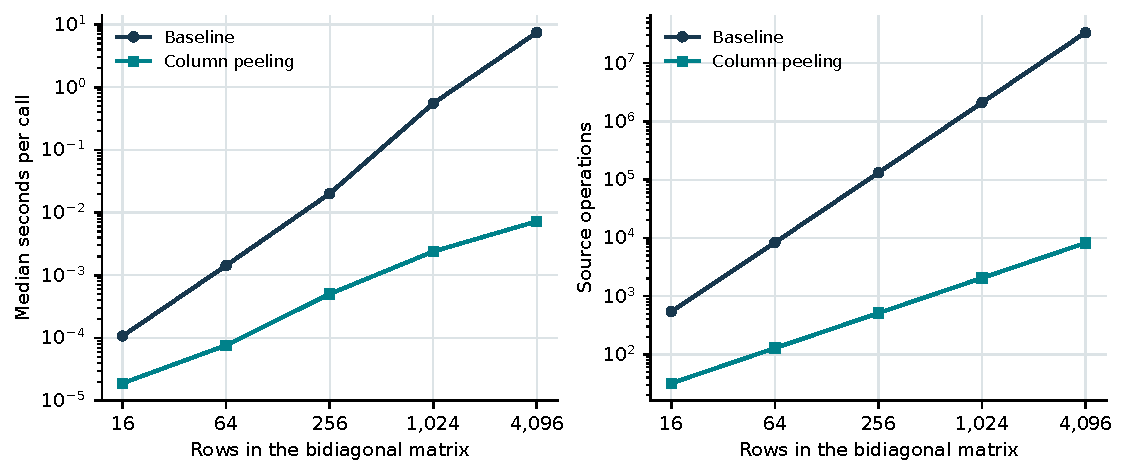
\includegraphics[width=\textwidth]{figures/cancellation_scaling.pdf}
\caption{The measured bidiagonal cancellation family. Left: five-trial
median producer times. Right: exact source-operation counters. Both axes
are logarithmic. The curves connect measured points; they are not fitted
claims about the full recognizer. The figure is regenerated directly
from the supplied benchmark JSON.}
\label{fig:scaling}
\end{figure}

The synthetic replay experiment uses conditional core incidence words,
not authenticated embedded three-dimensional sources. At 256 rows its
old median is 729.837 ms and its new median is 0.776 ms, a ratio of
$939.98\times$. This shows the cost removed by immutable timestamp replay
in the intended finite checker. It does not measure source authentication.

\subsection{Native timing: a small-kernel regression and almost unchanged queries}

The source-backed timing experiment separates prepared finite cores from
the entire old whole-cut query:
\begin{center}
\begin{tabular}{@{}p{.43\textwidth}rrr@{}}
\toprule
Scope & Baseline & New & Ratio\\
\midrule
All 106 prepared core producers & 4.807 ms & 6.515 ms & $0.738\times$\\
The 24 affected core producers & 1.397 ms & 0.974 ms & $1.435\times$\\
All 90 successful core replays & 7.084 ms & 5.703 ms & $1.242\times$\\
Complete 106-case old cut query & 36.515 s & 36.211 s & $1.008\times$\\
\bottomrule
\end{tabular}
\end{center}

The aggregate prepared-core timing is a regression: the new median is
about 35.6\% larger. This result must remain visible alongside the affected
subset's improvement. The samples vary, and such small calls are sensitive
to runtime overhead. The retained fast row-leaf path helps preserve
compatibility, but the data do not support a universal practical speedup.

The complete-query medians are effectively unchanged. Source orbit
construction, boundary observation and other work remain substantial;
the raw finite planner is too small a fraction of this corpus's full
query cost to transform the total. The synthetic thousand-fold ratio
must therefore not be advertised as an unknot-recognition speedup.
A next performance study should target authenticated source-query reuse
and boundary observation, while preserving this paired full-query scope.

\subsection{Seven additional geometric successes}

The saturated-bundle operator addresses coverage rather than simply
substituting a faster planner. Its final independent audit has the
following outcomes:
\begin{center}
\begin{tabular}{@{}lr@{}}
\toprule
Audit quantity & Count\\
\midrule
Supplied cuts & 106\\
Complete new whole-cut censuses & \textbf{85}\\
Earlier complete censuses retained & 78 of 78\\
New complete censuses & 7\\
Independent source-certificate replays & 85 of 85\\
Fresh Regina literal cuts completed & 99\\
Successful source censuses within literal-cut cap & 78\\
Agreement on those successful censuses & 78 of 78\\
Large-coordinate successes replayed without expansion & 7\\
Remaining joint raw stalls & 11\\
Remaining three-handle exclusions & 10\\
\bottomrule
\end{tabular}
\end{center}

All seven new cases previously returned \code{annular_core_attachment}.
All seven admit fresh literal cuts in Regina 7.4, and those independently
computed censuses agree with the new source proof. The seven successful
large-coordinate cases beyond the literal expansion cap are distinct
from these seven new cases; they are independently replayed but are not
claimed to have fresh expanded Regina comparisons.

In the following table $b$ is the number of base boundary components.
The listed genera are for the whole cut, with repeats indicating distinct
components. Genus zero denotes a ball.
\begin{center}\small
\begin{tabular}{@{}p{.39\textwidth}rlc@{}}
\toprule
Case & $T$ & Saturated nondisk base & Cut genera\\
\midrule
\path{pilot/fibonacci_lst_05/0} & 5 & M\"obius, $(\chi,b)=(0,1)$ & $1,2$\\
\path{pilot/fibonacci_lst_07/0} & 7 & M\"obius, $(0,1)$ & $1,2$\\
\path{pilot/fibonacci_lst_09/0} & 9 & M\"obius, $(0,1)$ & $1,2$\\
\path{pilot/lst_4_7/0} & 4 & M\"obius, $(0,1)$ & $1,2$\\
\path{pilot/lst_7_10/0} & 5 & M\"obius, $(0,1)$ & $1,2$\\
\path{fibonacci_lst_09/mixed} & 9 & One crosscap, $(-1,2)$ & $0,3,3$\\
\path{fibonacci_lst_10/mixed} & 10 & Annulus, $(0,2)$ & $0,2,2$\\
\bottomrule
\end{tabular}
\end{center}

The entire audit, including fresh oracle subprocesses, took 86.04 seconds.
That is a single mixed validation run, not a paired speed comparison
with the prior consumer. The package retains every case outcome,
refusal reason, source hash and fresh-oracle result. All 21 unresolved
cases remain inconclusive.

\subsection{Explicit witnesses for the remaining raw stalls}

The package also extracts all eleven remaining joint stopping sets.
For each case, the parallelity and boundary source proofs independently
replay before the exact matrix is read, and the separate obstruction
checker verifies the resulting nonempty row set. Six cases already have
an obstruction in their original-core row submatrix. In the other five,
that submatrix fully cancels and the obstruction requires the added
saturated relations. All five of those latter cases have saturated disk
bases, so the unresolved compatibility is already present in the
disk-absorption subproblem.

For example, \path{solid_torus_sum_rp3/mixed} has the stopping rows
$(8,10,11)$ on its nonzero stopping columns $(8,28,32)$, with matrix
\[
 \begin{pmatrix}2&1&1\\0&1&0\\0&0&1\end{pmatrix}.
\]
Every column sum is two. Its original-core row submatrix nevertheless
admits a full raw schedule. This small source witness makes the joint
compatibility issue concrete. It certifies a raw obstruction; it does
not infer the topology of that cut from an unsigned determinant or
from the triangulation's example name.

Exact uncapped matrices, row ownership, canonical stopping sets,
source-proof hashes and the old-core comparison are retained in
\path{artifacts/saturated/stopping_obstructions.json}. A portable
extractor reproduces them. These witnesses make the next investigation
of refused cases reproducible, while keeping unsupported topological
conclusions separate from algebraic ones.

\subsection{A complete small source example}

The smallest new example is \path{pilot/lst_4_7/0}. Its triangulation has
isomorphism signature \code{eHKPbcddhqxr} and four tetrahedra. Its normal
coordinates, in the source's seven-coordinate order per tetrahedron, are
\[
\begin{pmatrix}
1&1&1&1&0&0&0\\
1&1&1&1&0&0&0\\
1&1&0&0&1&0&0\\
0&0&0&0&0&2&0
\end{pmatrix}.
\]
The new saturated base is profile 0, a M\"obius band with one fully
attached annulus. It contributes one virtual band and relation row 5.
On original nonforest columns $(4,12,14,15,18,19,20,21)$, the exact
aggregate matrix, in row order $0,\ldots,5$, is
\[
 A=\begin{pmatrix}
 0&0&0&1&1&0&0&0\\
 0&0&0&0&0&1&0&0\\
 0&0&1&0&1&0&1&1\\
 0&0&0&1&0&1&1&1\\
 0&0&0&0&1&0&1&0\\
 1&2&0&0&0&0&0&0
 \end{pmatrix}.
\]
The omitted bundle column contains two in row 5 and zero in every other
row. The first five rows are the original core relations; they already
admit full cancellation when considered alone.
The verified source row/column schedule is
\[
(2,14),\ (5,4),\ (3,21),\ (0,15),\ (4,20),\ (1,19).
\]
The result consists of two components, of genera two and one. Their
Euler characteristics are $-1$ and $0$, summing to $-1$. Relation 5 is
cancelled at the second step using an old core column, while its virtual
band never appears in the stored matrix. This illustrates the exact
mechanism of the geometric extension on a genuine input.

The complete labelled tetrahedron gluings, source proofs, forest,
boundary charts, finite certificate and normal vector are in
\path{artifacts/saturated/certificates/019.json}. They determine the
source even if a different triangulation labelling is produced from
the isomorphism signature. The other six cases are recorded at the same
level of detail, rather than only by an expected genus or an example name.

\section{What the reduction contributes to the hierarchy goal}
\label{sec:hierarchy}

\subsection{A smaller exact local problem}

The saturated reduction replaces a potentially huge explicit relative
handle system by the matrix
\[
 A\in\NN^{(f+s)\times c},\qquad
 |\supp A|\le I_0+P.
\]
The new band handles affect genus counts and a geometric existence proof,
but they do not become cancellation choices. Complete source cancellation
is a deterministic sparse operation. A failure is accompanied by a
coordinate-dependent stopping obstruction to the entire raw rule.

These are useful improvements for a hierarchy implementation because they
give a precise accounting unit: the finite inherited core and active
interfaces, with numerical topological data kept in binary. They also
exclude an unproductive source of search. For a fixed matrix, branching
over its positive raw pivot orders or proposed survivors cannot discover
a full cancellation when the complete column test fails.

The result is not a bound on how many different matrices a hierarchy must
visit. A new normal surface, a different disk system or a genuinely
intersection-reducing move can change the stopping set. Controlling those
changes remains a geometric question.

\subsection{A precise global accounting criterion}

It is helpful to state a global cost target in a form that does not confuse
deterministic work with branching. The following elementary search-tree
lemma is an accounting device, not a new unknot-recognition theorem.

\begin{lemma}[Branch-product bound]\label{lem:branch-product}
Let a finite rooted search tree have maximum depth $D$. At an internal
vertex $v$, let $b(v)\ge1$ be its number of children. Suppose every
root-to-leaf path satisfies
\[
 \sum_{v\text{ on the path}}\log_2 b(v)\le K.
\]
Then the tree has at most $2^K$ leaves and at most $(D+1)2^K$ vertices.
\end{lemma}

\begin{proof}
Start with mass one at the root and divide each vertex's mass equally
among its children. A leaf receives
$\prod_v b(v)^{-1}\ge2^{-K}$, while the leaf masses sum to one. Thus
there are at most $2^K$ leaves. Every vertex lies on some root-to-leaf
path, and the union of those paths has at most $(D+1)$ vertices per leaf.
\end{proof}

\Needspace{14\baselineskip}
\begin{theorem}[A sufficient quasi-polynomial integration contract]
\label{thm:global-contract}
Suppose a complete deterministic recognition procedure on an $n$-crossing
diagram has a finite search tree with the following properties:
\begin{enumerate}
\item Every explored state, source certificate and transported boundary
pattern has encoded size at most $n^a$ for a fixed constant $a$.
\item Each node's full processing cost, including source construction,
all rejected local candidates and independent local certification, is
polynomial in $n$.
\item The depth is polynomial in $n$, and the sum of $\log_2 b(v)$ along
every root-to-leaf path is $O((\log n)^2)$.
\item Every terminal conclusion is sound, and the search covers all
required alternatives, so completed exhaustion justifies its negative
conclusions.
\end{enumerate}
Then the procedure runs in $n^{O(\log n)}$ bit time. The cancellation
operators developed in this report satisfy a polynomial local-cost
requirement once their authenticated source data is available.
\end{theorem}

\begin{proof}
Lemma~\ref{lem:branch-product} bounds the node count by
$\poly(n)2^{O((\log n)^2)}=n^{O(\log n)}$. Multiplying by the
polynomial per-node bit cost preserves this bound. The last hypothesis
supplies decision correctness. The finite cancellation bound follows
from Theorems~\ref{thm:linear} and~\ref{thm:saturated-even-columns},
Proposition~\ref{prop:compiled-size}, and polynomial binary arithmetic
for the census.
\end{proof}

The hypotheses are intentionally explicit. They have \emph{not} been proved
for the maintained general recognizer. A polynomial number of deterministic
steps along a branch would be harmless under this contract; an uncontrolled
number of branching choices or a large rebuild cost would not be. Binary
compression of one supplied cut addresses only part of the first two items.

Lackenby's hierarchy work provides the mathematical framework for further
development\cite{lackenby-2026,lackenby-talk}. Efficient existence and
verification statements must be distinguished from finding the desired
surface and from bounding all unsuccessful work. A short certificate
does not by itself give a comparably fast deterministic producer.

\subsection{Remaining obligations with concrete failure modes}

\paragraph{Surface coverage.}
A supplied-cut census says nothing about whether a producer can find a
useful surface within a small collection of sectors. Dense normal vectors
and large coordinates may be perfectly manageable once supplied; they
can still be difficult to discover. A complete theorem must quantify
the entire candidate set, including rejected candidates.

\paragraph{Marked transport.}
The new proof establishes an unmarked homeomorphism type and raw
incidence properties. A later hierarchy step needs the inherited
boundary pattern as embedded curves and graphs. Unsigned passenger
transport supplies exact numerical data under its update rule, but
does not retain cyclic order or identify which endpoints join. These
missing data can affect essentiality of a terminal pattern.

\paragraph{Escaping a raw stopping set.}
Example~\ref{ex:unimodular} shows that even a ball can have a blocked
chosen raw system. A complete algorithm therefore needs operations that
can lower actual geometric intersections or change the chosen source
decomposition. Pure positive pivots cannot do this. The required repair
cost must be bounded on all instances, not inferred from a successful
finite corpus.

\paragraph{Three-handles and closed bases.}
The present consumer excludes both. A source core with a three-handle
does not become simpler merely because its boundary genera are known.
A valid extension requires actual geometric removals or a separate
certified topological argument.

\paragraph{State identity and restarts.}
The canonical stopping set belongs to one labelled source matrix.
It does not provide canonical representatives of embedded handle
structures. Memoization can be sound only if its keys retain the
needed geometric and marking information. Rebuilding after a
compression or changing the forest can introduce new states; their
number and encoded sizes must be included in the global sum.

\paragraph{Diagram provenance and final decisions.}
The normal-cut source contracts bind a triangulation and normal vector.
They do not independently bind an arbitrary diagram to that exterior.
The exact full recognizer retains its existing routes and fallback.
The experimental APIs in this package issue supplied-cut results, not
new standalone knot verdicts.

\subsection{A realistic next milestone}

The most direct continuation is a \emph{marked} version of the complete
column certificate. Its no-fill order has immutable donors and a directed
acyclic dependency graph. This removes uncertainty about pivot discovery
and limits numerical growth, allowing the geometric work to focus on
transporting embedded strand data through a fixed successful schedule.

A useful milestone would accept an authenticated source core and a finite
marked pattern, produce the entire surviving marked handlebody structure,
and independently replay every strand attachment without expanding large
parallel families. Combining that with one fully certified next hierarchy
cut would demonstrate a genuine transition, rather than another isolated
topological census. It would still need a global coverage and branching
argument to achieve the quasi-polynomial target.

\section{Further research questions and proposed next work}
\label{sec:research}

The following questions are ordered by how directly they build on the
proved and implemented results. Each asks for a concrete mathematical
or computational advance, with a criterion by which progress can be assessed.

\subsection{Transport an embedded boundary pattern through a no-fill schedule}

Can the immutable donor structure be lifted from unsigned rows to ordered
strand systems on the boundary of the handlebody? The input should specify
actual source endpoints, local cyclic orders and fibre transport, not only
intersection counts. The output should encode the induced pattern after
each geometric cancellation or directly on the final handlebody.

The passenger theorem bounds the growth of numerical counts. The unresolved
issue is the geometry of their concatenation. A successful result should
give a polynomial bound on the size of a shared representation and an
independent replay theorem. Small counterexamples with equal incidence
and different boundary order should be part of the validation set.

\subsection{Give saturated bands a compressed marked realization}

The saturated theorem omits a potentially enormous family of even band
columns because they cannot be pivots. Can one retain those bands as a
small typed family while transporting specified markings through them?
The target is a source-certified relative band system, with attachment
addresses and cyclic order, whose encoding is polynomial in the source
and the bit length of the base topology.

An abstract free-group presentation with a large product of commutators
does not settle this geometric problem. The representation should support
both orientable and nonorientable bases and arbitrary compatible annular
gluing twists. The punctured-torus and M\"obius examples provide elementary
test cases, while the seven new source cuts provide native regression cases.

\subsection{Identify small repairs of a raw stopping core}

Which geometric moves destroy a specified stopping set by decreasing
actual intersections? The persistence theorem proves that searching more
positive pivot orders cannot help. A useful repair theorem would identify
a bounded-size configuration in every blocked core belonging to a
specified topological class and supply a verified transformation that
reduces a stated potential.

The class should be restricted first. For example, study layered solid
tori or source cuts with a bounded number of saturated relations. The
goal is a theorem with explicit dependence on the chosen parameter,
not a promise inferred from random small examples. The blocked ball
matrix $\left(\begin{smallmatrix}1&1\\1&2\end{smallmatrix}\right)$ is the
first required test: a useful repair can undo a handle slide, but no
positive raw pivot order can finish it.

\subsection{Optimize the choice of source forest with certified scope}

Our completeness theorem fixes the core forest. How does
$\Stop(A)$ change when a tree edge is exchanged with a nonforest edge?
An incremental exact incidence update could avoid reconstructing the
entire source for every forest. The difficult part is to prove the
geometric cocore correspondence and to bound a complete family of
forests or exchanges.

A practical first deliverable is a source-certified one-edge exchange
with an independently verified new aggregate matrix. A later theorem
could characterize a class in which polynomially many exchanges expose
full raw cancellation. The mere existence of a successful forest does
not give a fast complete search over all forests.

\subsection{Use a stopping certificate to focus higher-level moves}

The residual is a canonical row set in a fixed matrix. Can repair proposals
be restricted to neighborhoods of that set while preserving completeness?
One possibility is to keep a typed incidence graph containing its rows,
their columns and the nearby geometric charts. A theorem would need to
show that irrelevant regions can be retained by identity while a useful
repair is found inside the selected region.

This is a locality question about geometric simplification, not a
consequence of the algebraic stopping condition alone. Its benefit would
be a smaller complete move neighborhood with an explicit certificate of
unchanged exterior data.

\subsection{Extend the consumer to three-handle cores}

Ten cuts in the retained audit still have core three-handles. Can a dual
source peeling rule identify geometric two/three-handle cancellations
without flattening the compressed cut? A suitable rule must authenticate
the attaching sphere and its unique intersection, rather than treating
an algebraic incidence as sufficient.

Begin with cases where a genuine free face is present and record its
effect on all interface charts. Then investigate whether a bounded
sequence of dual moves covers a useful larger class. Every accepted
reduction should have an independent source replay and preserve the
component census used by the present implementation.

\subsection{Resolve the eleven remaining raw stalls}

The source audit gives eleven cuts with a failed combined raw system.
Their exact canonical stopping witnesses are included: six obstructions
already lie in the original core, and five require added saturated disk
relations. Classify the geometry behind those witnesses: shared annular
powers, interacting original two-handles, graph cycles, or another
configuration. This is a finite, concrete next experiment.

The desired output is not merely a longer list of heuristic moves. It
is a small set of proved geometric lemmas, each supported by source
certificates, that either resolves a family of stalls or explains why
a new surface or disk system is needed. Some test cuts may actually
fail to be handlebodies; in those cases a separate authenticated
topological obstruction is the appropriate goal. Any cases still
unsupported should remain inconclusive.

\subsection{Unify geometric source compilation with the incoming interface kernels}

The moment-coded first-return report compresses boundary observations,
while the present operator consumes their ordered annular words. Can the
source proofs be reused without changing their trust boundary, reducing
the repeated orbit-query cost that dominates small examples?

The interface contract must preserve shared corners, actual gaps,
orientation transport, whole-circle detection and port ownership. A
useful implementation should retain the old query as a differential
oracle and record both complete-query and finite-kernel timings. This
question is promising precisely because the current empirical evidence
does not show a broad whole-query speedup from the new core planner alone.

\subsection{Find a useful-surface coverage theorem with an explicit budget}

Can every nonterminal member of a restricted hierarchy class be advanced
by a surface whose active interface, saturated residue and repair cost
have a provable bound? Candidate parameters include the number of
saturated relations and the geometry of their stopping core. A useful
theorem should specify how the surface is found, how failures are
charged and how the inherited pattern is transported.

An existence theorem without a producer or an upper bound on failed
candidates is insufficient for the running-time target. Conversely, a
complete producer on a clearly defined restricted class would already
be a substantial result, even before extension to all knot exteriors.

\subsection{Prove a global branching and state-size potential}

Find a potential controlling branching, resets and encoded state size.
Theorem~\ref{thm:global-contract} asks for an $O((\log n)^2)$ path
branching budget with polynomial depth and per-state work.

The potential must include boundary patterns, geometric repairs and
source rebuilding. A raw stopping core alone cannot suffice: coordinate
changes can create or remove it. Proving this combined bound is the
principal remaining step toward a general $n^{O(\log n)}$ recognizer.

\clearpage
\begin{thebibliography}{99}
\raggedright
\addcontentsline{toc}{section}{References}

\bibitem{repo}
Vladimir Reshetnikov and contributors,
\emph{ProveIt: Topology/UnknotRecognition}, source repository,
revision \texttt{704600626606a9097cfd89d4e3d2bbc63c8dd1cb},
inspected 12 October 2026.
\url{https://github.com/VladimirReshetnikov/ProveIt/tree/704600626606a9097cfd89d4e3d2bbc63c8dd1cb/Topology/UnknotRecognition}.

\bibitem{incoming}
ProveIt incoming research archives, 12 October 2026:
\emph{Disconnected Tile Kernels},
\emph{Moment Coded First Returns},
\emph{Unknot Hierarchy Kernels}, and
\emph{Unknot Sparse Cut Grammars}.
Exact archive names and hashes are retained in this package's provenance files.
\url{https://github.com/VladimirReshetnikov/ProveIt/tree/704600626606a9097cfd89d4e3d2bbc63c8dd1cb/docs/incoming}.

\bibitem{hierarchy-incoming}
\emph{ProveIt Unknot Hierarchy Kernels}, incoming research package,
\path{ProveIt_Unknot_Hierarchy_Kernels_2026-10-12.zip},
12 October 2026. Relative-handle results for nonsaturated and saturated
bordered interval bundles. See the pinned incoming directory in
reference~\cite{incoming}; archive SHA-256 begins \texttt{e5ab7d2a3d0eca30}.

\bibitem{lackenby-talk}
Marc Lackenby,
\emph{Unknot recognition in quasi-polynomial time},
February 2021 talk slides, 109-page version linked by the project;
main quasi-polynomial theorem on slides 13--14.
\url{https://people.maths.ox.ac.uk/lackenby/quasipolynomial-talk.pdf}.

\bibitem{lackenby-oxford}
Marc Lackenby,
\emph{Unknot recognition in quasi-polynomial time},
Oxford talk handout, March 2021, 34 pages; main theorem on slide 7.
\url{https://people.maths.ox.ac.uk/lackenby/quasipolynomial-talk-oxford-compressed.pdf}.
See also the Oxford announcement:
\url{https://www.maths.ox.ac.uk/node/38304}.

\bibitem{lackenby-2026}
Marc Lackenby,
\emph{Incompressible surfaces, hierarchies and unknot recognition},
arXiv:2607.23350v1 [math.GT], 25 July 2026.
\url{https://arxiv.org/abs/2607.23350v1}.
The supplied project also contains the source of this version under
\path{docs/arXiv-2607.23350v1} within the unknot-recognition subtree.

\bibitem{richardson-urbanke}
Thomas J. Richardson and R{\"u}diger L. Urbanke,
``Efficient Encoding of Low-Density Parity-Check Codes,''
\emph{IEEE Transactions on Information Theory} \textbf{47}(2)
(2001), 638--656. Appendix C, p.~655.
\url{https://www.csie.ntu.edu.tw/~mku/research/LDPC/asset/papers/encode/efficient_encode_LDPC.pdf}.

\bibitem{di-et-al}
Changyan Di, David Proietti, I. Emre Telatar, Thomas J. Richardson,
and R{\"u}diger L. Urbanke,
``Finite-Length Analysis of Low-Density Parity-Check Codes on the Binary
Erasure Channel,''
\emph{IEEE Transactions on Information Theory} \textbf{48}(6)
(2002), 1570--1579.
\href{https://doi.org/10.1109/TIT.2002.1003839}{doi:10.1109/TIT.2002.1003839}.
Primary paper copy:
\url{https://cnls.lanl.gov/~chertkov/Papers/02DPTRU.pdf}.

\bibitem{urm}
Martin C. Golumbic, Tirza Hirst, and Moshe Lewenstein,
``Uniquely Restricted Matchings,''
\emph{Algorithmica} \textbf{31}(2) (2001), 139--154.
\href{https://doi.org/10.1007/s00453-001-0004-z}{doi:10.1007/s00453-001-0004-z}.
\url{https://research.ibm.com/publications/uniquely-restricted-matchings}.

\bibitem{schultens-weidmann}
Jennifer Schultens and Richard Weidmann,
``Destabilizing amalgamated Heegaard splittings,''
\emph{Geometry \& Topology Monographs} \textbf{12} (2007), 319--334.
\href{https://doi.org/10.2140/gtm.2007.12.319}{doi:10.2140/gtm.2007.12.319}.
Definition 6 and Lemma 24 in the published version.
\url{https://arxiv.org/abs/math/0510386}.

\end{thebibliography}

\appendix
\section{Package contents, integration, and reproduction}
\label{sec:reproduction}

\subsection{Layout and source identity}

The archive is rooted at
\path{ProveIt_Unknot_Stopping_Cores_2026-10-12/}.
Its top-level README describes the recommended integration order and
the scope of each API. The important directories are:
\begin{description}[style=nextline,leftmargin=1em]
\item[\path{article/}]
This article's complete TeX sources, reference list, compiled PDF,
vector and raster figure, figure-generation script and build script.
\item[\path{integration/}]
A repository-relative patch, complete updated source files, old/new
file hashes and checked integration instructions. Existing code changes
are limited to the core producer and verifier; the saturated and
passenger APIs are added modules.
\item[\path{artifacts/column_cancellation/}]
The complete paired benchmark JSON and focused test log.
The reproducible benchmark driver and exact baseline modules are part
of the repository integration overlay.
\item[\path{artifacts/saturated/}]
The full 106-case audit, environment, source provenance, exact seven
new cases and their source certificates, the worked matrix for case 019,
focused test log and portable audit driver.
\item[\path{artifacts/validation/}]
The complete maintained-suite log, separate passenger test log and
validation summary.
\item[\path{artifacts/source/}]
The exact retained 106-case corpus, previous primitive-annulus audit,
and their provenance hashes.
\end{description}

The source integration targets repository revision
\begin{center}\texttt{704600626606a9097cfd89d4e3d2bbc63c8dd1cb}.\end{center}
A later revision
requires reviewing the affected interfaces and replaying the retained
evidence. The package does not include a duplicate repository checkout.
Its patch was checked against exact pinned base files in an isolated
tree. The complete replacements provide a convenient second way to
inspect every proposed source change.

\subsection{Apply and validate the source changes}

Let \code{PROVEIT_CHECKOUT} be the root of a checkout at the pinned
revision, and \code{RESEARCH_PACKAGE} the root of this unpacked package.
Review \path{integration/README.md} and its old/new hash manifest first.
The essential Git operations, run from the checkout root, are:
\begin{lstlisting}
git apply --check "$RESEARCH_PACKAGE/integration/integration.patch"
git apply "$RESEARCH_PACKAGE/integration/integration.patch"
\end{lstlisting}
These commands are provided for the maintainer's integration workflow.
This research run made no remote commit or repository publication.

Run the tests from
\path{Topology/UnknotRecognition/fast} in the patched checkout:
\begin{lstlisting}
python3 -m unittest tests.test_column_cancellation \
    tests.test_normal_cut_saturated \
    tests.test_raw_passenger_transport -v
python3 -m unittest discover -s tests
\end{lstlisting}
The finite producer and replay code use Python's standard library and
the existing ProveIt modules. The maintained repository's broader tests
and oracle comparisons retain their existing dependency requirements.
The retained fresh literal-cut audit used Regina 7.4.

\subsection{Reproduce the paired benchmark}

From the same \path{fast} directory:
\begin{lstlisting}
python3 benchmark_column_cancellation.py \
    --trials 5 --output reproduced-column-cancellation.json
\end{lstlisting}
The driver locates its baseline modules and corpus relative to its own
file. It compares the same source cores and verifies the successful
results before recording timings. The optional
\code{--skip-whole-cuts} flag is useful for a finite-kernel-only
experiment, but such a run cannot reproduce the complete-query row in
the article's table. The largest synthetic baseline and the complete
query make the full experiment appreciably longer than a unit test.

Timing samples are environment-dependent. Reproduction should confirm
the algebraic outcomes, source censuses and operation counters; it need
not reproduce the saved wall-clock numbers digit for digit. A proposed
optimization should retain both affected-subset and all-case timings,
including regressions.

\subsection{Reproduce the saturated source audit}

The packaged driver accepts an explicit checkout path:
\begin{lstlisting}
python3 "$RESEARCH_PACKAGE/artifacts/saturated/run_audit.py" \
    --checkout "$PROVEIT_CHECKOUT" --fresh-oracles \
    --output reproduced-saturated/audit.json
\end{lstlisting}
It reruns the source producer, disables producer entry points during
independent replay, preserves earlier successes, and invokes the
maintained Regina literal-cut oracle subject to its expansion cap.
Omitting \code{--fresh-oracles} uses the historical comparison packets
while still rerunning the new source pipeline. The output directory is
separate from the retained audit by default.

For a single retained certificate, use the source wrapper's verifier:
\begin{lstlisting}[language=Python]
import json
from fastunknot.normal_cut_saturated_verify import \
    verify_normal_cut_saturated

with open("/path/to/certificates/019.json") as source:
    case = json.load(source)
assert verify_normal_cut_saturated(
    case["triangulation"], case["coordinates"],
    case["certificate"])
\end{lstlisting}
The certificate contains the labelled source gluings. No inference from
the isomorphism signature or from the expected genus is needed.

\Needspace{13\baselineskip}
\subsection{Call the new operators}

The saturated wrapper is opt-in:
\begin{lstlisting}[language=Python]
from fastunknot.normal_cut_saturated import normal_cut_saturated
from fastunknot.normal_cut_saturated_verify import \
    verify_normal_cut_saturated

answer = normal_cut_saturated(
    triangulation, coordinates, record_certificate=True)
if answer["status"] == "COMPLETE":
    assert verify_normal_cut_saturated(
        triangulation, coordinates, answer["certificate"])
    histogram = answer["census"]["histogram"]
\end{lstlisting}
The lower-level \code{saturated_source_census} is conditional on
already authenticated geometry, base summaries and an ordered boundary
skeleton. The wrapper supplies that authentication.

For exact count transport after a complete column schedule:
\begin{lstlisting}[language=Python]
from fastunknot.core_handlebody import column_cancellation_plan
from fastunknot.raw_passenger_transport import transport_raw_passenger

counts = {0: {0: 1, 1: 2, 2: 3},
          1: {1: 1, 3: 5}, 2: {2: 1, 3: 7}}
plan = column_cancellation_plan(counts)
passenger = transport_raw_passenger(
    counts, plan["cancellations"], {0: 11, 3: 13})
assert passenger == {3: 354}
\end{lstlisting}
The original exact \code{counts} must be supplied, not a capped copy.
The operation verifies its donor schedule but does not authenticate
embedded passenger geometry.

\subsection{Build the article and figure}

From any working directory, run
\begin{lstlisting}
python3 /path/to/package/article/build.py
\end{lstlisting}
The script uses \code{latexmk} when available and otherwise runs
\code{pdflatex} three times. It needs a standard TeX installation with
the packages named in the source. All included figure files are already
built. To regenerate them from the retained benchmark JSON, run
\code{article/make_figures.py} with Matplotlib installed, then rebuild
the article. The delivered PDF was compiled, checked for unresolved
references and layout defects, rendered, and visually inspected.

\subsection{Interpretation and integration limits}

The patch upgrades raw planning and replay, and adds a broader positive
source-cut census. It does not change the recognizer's dispatcher or
its exact fallback policy. A caller must preserve \code{INCONCLUSIVE}
as an unsupported or unfinished result. A stopping-set certificate
excludes only a complete raw schedule in its named source matrix.

The next integration milestone is to preserve embedded boundary data
through these complete schedules and certify a subsequent hierarchy
transition. The present article supplies precise local theorems,
implementations and evidence on which that work can build; the global
quasi-polynomial claim remains a research objective.

\end{document}
